\begin{figure}[H]
\centering
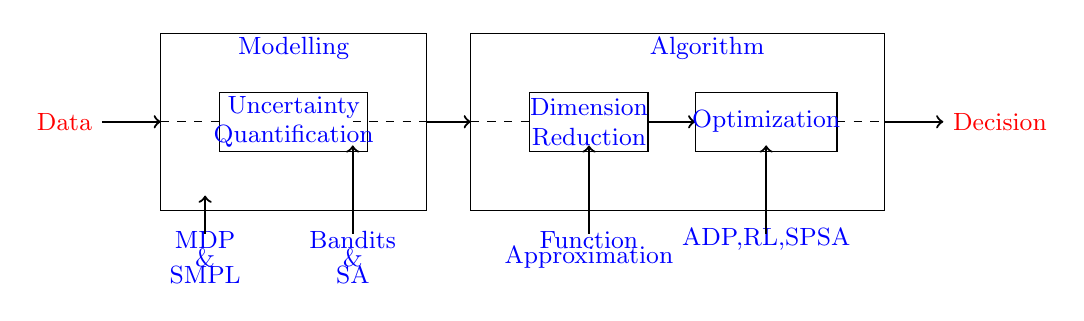
\begin{tikzpicture}[scale=0.75,font=\small,axis/.style={very thick, ->}]
\draw [black](-2.25,-1) rectangle (2.25,2);
\node[blue] at(0,1.75) {Modelling};
\node[blue] at(-1.5,-1.5) {MDP};
\node[blue] at(-1.5,-1.8) {\&};
\node[blue] at(-1.5,-2.1) {SMPL};
\draw[thick,->](-1.5,-1.4)--(-1.5,-0.75);


\node[blue] at(1,-1.5) {Bandits};
\node[blue] at(1,-1.8) {\&};
\node[blue] at(1,-2.1) {SA};

\draw[thick,->](1,-1.4)--(1,0.1);

\node[blue] at(5,-1.5) {Function};
\node[blue] at(5,-1.8) {Approximation};
\draw[thick,->](5,-1.4)--(5,0.1);

\node[blue] at(8,-1.5) {ADP,RL,SPSA};
%\node[blue] at(8,-1.8) {\&};
%\node[blue] at(8,-2.1) {RL};

\draw[thick,->](8,-1.4)--(8,0.1);

\draw [black](-1.25,0) rectangle (1.25,1);
\node[blue] at(0,0.75) {Uncertainty};
\node[blue] at(0,0.25) {Quantification};

\draw[thick,->](-3.25,0.5)--(-2.25,0.5);
\draw[dashed,-](-2.25,0.5)--(-1.25,0.5);


\draw[dashed,-](1,0.5)--(2.25,0.5);
\draw[thick,->](2.25,0.5)--(3,0.5);
\draw[dashed,-](3,0.5)--(4,0.5);



\draw [black](3,-1) rectangle (10,2);
\node[blue] at(7,1.75) {Algorithm};
\draw [black](4,0) rectangle (6,1);
\node[blue] at(5,0.75) {Dimension};
\node[blue] at(5,0.25) {Reduction};

\draw[thick,->](6,0.5)--(6.8,0.5);
\draw[dashed,-](9.2,0.5)--(10,0.5);
\draw[thick,->](10,0.5)--(11,0.5);
\node[red,right] at(11,0.5) {Decision};
\node[red,left] at(-3.25,0.5) {Data};


\draw [black](6.8,0) rectangle (9.2,1);
\node[blue] at(8,0.5) {Optimization};

\end{tikzpicture}
\captionsetup{font=footnotesize}
\captionof{figure}{The figure shows the various steps starting with \emph{data}, followed by \emph{modelling} and then by \emph{algorithm} leading to the \emph{decision rule} . The modelling step involves \emph{uncertainty quantification} and the algorithmic step can further be split into \emph{dimensionality reduction} and \emph{optimization}. Markov Decision Processes (MDPs) and Stochastic Max-Plus (SMPL) system are useful mathematical models of uncertainty. Multi-arm bandit and Stochastic Approximation (SA) theories helps us in uncertainty quantification. Function approximation techniques are used to address the curse-of-dimensionality. \emph{Approximate Dynamic Programming} (ADP), \emph{Reinforcement Learning} (RL) and \emph{Simultaneous Perturbation Stochastic Approximation} (SPSA) algorithms are optimization routines that eventually lead to the final decision rule.
}
\end{figure}

